\documentclass[10pt,a4paper]{article}
\usepackage[utf8]{inputenc}
\usepackage{amsmath}
\usepackage{amsfonts}
\usepackage{amssymb}
\usepackage{graphicx}
\usepackage{caption}
\author{Antonin Garret et Raphael Truffet}
\title{Projet : Ants vs SomeBees}
\date{}
\renewcommand{\contentsname}{Sommaire}

\begin{document}

\maketitle
\tableofcontents
\newpage

\section*{Introduction}

Dans ce projet, nous avons programmé un jeu intitulé "Ants vs SomeBees", inspiré du jeu "Plants vs Zombies". L'intérêt principal de ce projet était de découvrir la programmation orientée objet. Cela nous a donc amené à faire des choix de programmation de façon à exploiter au maximum cet aspect là.

\section{Dépendances entre classes}
\subsection{Diagramme de classes}

\begin{center}
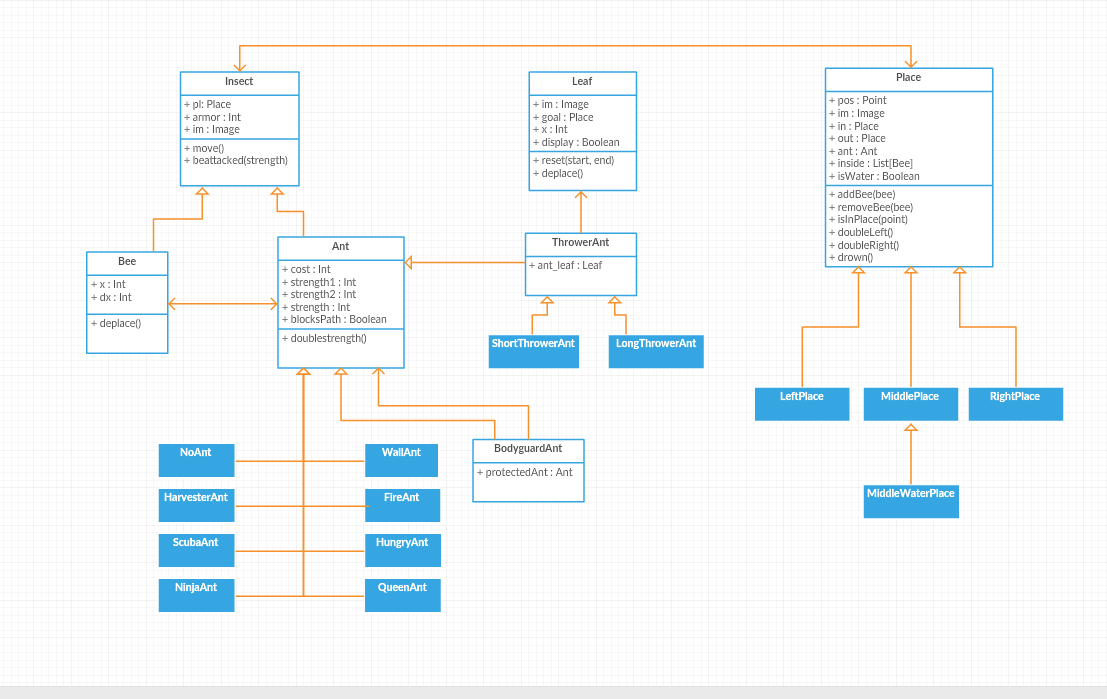
\includegraphics[scale=0.3]{ClassDiagram}
\captionof{figure}{Diagramme UML}
\label{ClassDiagram}
\end{center}

Le diagramme est également en annexe dans un format plus adapté

\subsection{Commentaires}

La programmation orientée objet a bien entendu ses avantages, comme par exemple le fait que les informations sur un objet soient regroupées. Cependant, cela peut également amener à des situations particulières, par exemple, on peut remarquer que la classe Ants contient un champ qui indique la place où se trouve la fourmi (en héritage de la classe Insect) mais aussi que la classe Place contient un champ qui indique quelle fourmi s'y trouve (cette fourmi étant une fourmi "nulle", appelée NoAnt, si la Place est considérée vide dans le jeu). L'information est donc stockée en double. On y perd lors de la création et des modifications de l'information, mais on y gagne en clarté du code et en rapidité lorsque l'on souhaite seulement accéder aux informations, ce qui est plus fréquent.

L'héritage entre les classes a permit de factoriser un bonne partie du code et de limiter la taille des pattern matching.

\section{Graphisme}

\subsection{Affichage}

Ici encore, la notion de classes a été pratique. En effet, chaque classe contenait un champ qui stocke son image. Dès lors, il suffit de parcourir tous les objets et de placer l'image à sa position (pour les insectes, la position est connue à travers le champs de place). 

\subsection{Animation fluide}
  
Le jeu se joue au tour par tour, alors que les animations sont continues (pour les feuilles et les abeilles). Il a donc fallu gérer cette contradiction. L'idée a été de rajouté pour ces objets un champ pour indiquer sa position qui est mis à jour à chaque frame. Cette position n'est modifiée que si l'objet doit se déplacer, or cette information n'est modifiée que lorsque l'on change de tour. Dès lors, on utilise un champ qui indique la distance qu'il reste à parcourir, qui est augmenté lorsqu'un déplacement est commandé, et diminué lorsque l'objet se déplace effectivement.

\section{Interactions avec l'utilisateur}
Le but du projet étant de créer un jeu auquel il soit possible de jouer sur un ordinateur, il nous fallait implémenter des méthodes qui permettent à un utilisateur d'influer sur le déroulement du jeu. Les principales actions devant être possibles pour l'utilisateur sont :
\begin{itemize}
  \item ajouter et supprimer des fourmis sur la table de jeu
  \item passer au tour suivant
\end{itemize}

Pour réaliser ces méthodes, nous avons utilisé la méthode listenTo de la bibliothèque ScalaSwing.

Pour l'ajout et la suppression de fourmi, nous avons ajouté une méthode sur la classe Place prenant un point en argument, qui renvoit un booléen indiquant si le point et dans la Place ou non. Cette méthode nous permet donc de repérer dans quelle Place est le pointeur de souris quand l'utilisateur fait un clic. Nous avons ensuite créé des Places qui représentent un "marché", et qui contiennent chacune un type de fourmi. Si l'utilisateur clique sur une de ces Places, le jeu vérifient qu'il dispose d'assez de nourriture pour créer une fourmi de ce type (et, dans le cas d'une reine, s'il n'existe pas déjà une fourmi de ce type), et stocke si c'est le cas le type de fourmi dans un champ currentAnt. Si l'utilisateur clique ensuite sur une Place de la table de jeu, le jeu crée une fourmi du type de currentAnt sur cette Place, et réinitialise currentAnt. Si l'utilisateur souhaite supprimer une fourmi, il dispose dans le marché d'une Place contenant le type NoAnt.

Pour que l'utilisateur passe au tour suivant, il lui suffit d'appuyer sur le bouton N du clavier, comme le lui indique une phrase sur l'interface graphique. 


\section*{Conclusion}

La programmation orientée objet s'est avérée adaptée pour la programmation d'un jeu, et le langage utilisé, Scala, permettait cette utilisation. Même si des améliorations restent possibles, comme la synchronisation de la disparition des abeilles avec la collision avec les feuilles ou changer l'image de Hungry Ant après qu'elle ait mangé, le résultat est jouable. De plus, un autre avantage de la programmation orientée objet est que le jeu peut être complété et modifié sans avoir à transformer tout le code. Ces modifications pourront donc être apportées sans trop de difficultés.

\end{document}
